\documentclass{standalone}
\usepackage{graphicx}	
\usepackage{amssymb, amsmath}
\usepackage{color}

\usepackage{tikz}
\usetikzlibrary{intersections, backgrounds}

\definecolor{light}{RGB}{220, 188, 188}
\definecolor{mid}{RGB}{185, 124, 124}
\definecolor{dark}{RGB}{143, 39, 39}
\definecolor{highlight}{RGB}{180, 31, 180}
\definecolor{gray10}{gray}{0.1}
\definecolor{gray20}{gray}{0.2}
\definecolor{gray30}{gray}{0.3}
\definecolor{gray40}{gray}{0.4}
\definecolor{gray60}{gray}{0.6}
\definecolor{gray70}{gray}{0.7}
\definecolor{gray80}{gray}{0.8}
\definecolor{gray90}{gray}{0.9}
\definecolor{gray95}{gray}{0.95}

\newcommand*{\offset}{0.025}

\begin{document}

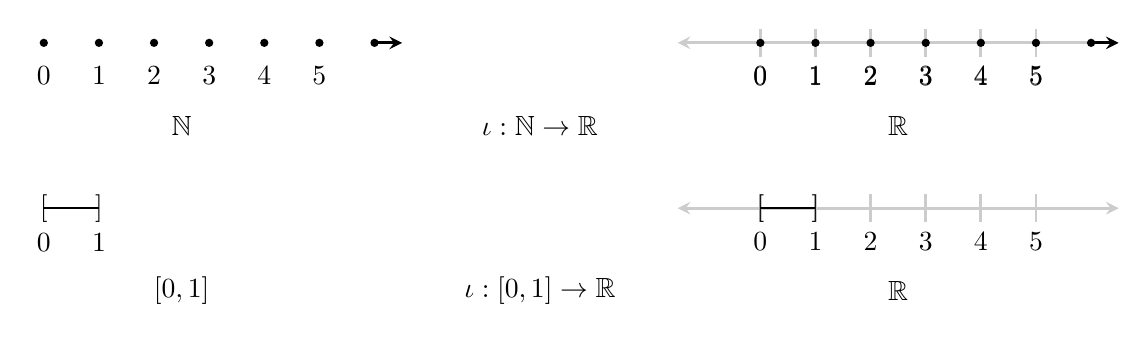
\begin{tikzpicture}[scale=0.35, thick]

  \foreach \i in {0, 1, ..., 5} {
    \fill [] (2 * \i - 18, 0) circle(0.15)
    node[below, yshift=-5] { $\i$ };
  } 
  \fill [] (-6, 0) circle(0.15); 
  \draw [->, >=stealth, line width=1, color=black] (-6, 0) -- +(1, 0);
  
  \node[] at (-13, -3) { $\mathbb{N}$ };
  
  \node[] at (0, -3) { $\iota: \mathbb{N} \rightarrow \mathbb{R}$ };

  \draw [<->, >=stealth, line width=1, color=gray80] (5, 0) -- +(16, 0);
  \node[] at (13, -3) { $\mathbb{R}$ };
  
  \foreach \i in {0, 1, ..., 5} {
    \draw [line width=1, color=gray80, text=black] (2 * \i + 8, 0.5) -- +(0, -1)
    node[below] { $\i$ };
  }  
  \fill [] (20, 0) circle(0.15); 
  \draw [->, >=stealth, line width=1, color=black] (20, 0) -- +(1, 0);
  
  
  \foreach \i in {0, 1, ..., 5} {
    \fill [] (2 * \i + 8, 0) circle(0.15)
    node[below, yshift=-5] { $\i$ };
  }  
  
  %
  \draw[-] (-18, -6) -- (-16, -6);
  \node at (-18, -6) {$[$};
  \node at (-18, -7.25) {$0$};
  \node at (-16, -6) {$]$};
  \node at (-16, -7.25) {$1$};
  
  \node at (-13, -9) { $[0, 1]$ };
  
  \node at (0, -9) { $\iota: [0, 1] \rightarrow \mathbb{R}$ };

  \draw [<->, >=stealth, line width=1, color=gray80] (5, -6) -- +(16, 0);
  \node[] at (13, -9) { $\mathbb{R}$ };
  
  \foreach \i in {0, 1, ..., 5} {
    \draw [line width=1, color=gray80, text=black] (2 * \i + 8, -5.5) -- +(0, -1)
    node[below] { $\i$ };
  }  
  
  \draw[-] (8, -6) -- (10, -6);
  \node at (8, -6) {$[$};
  \node at (10, -6) {$]$};
  
\end{tikzpicture}

\end{document}  